%----------------------------------------------------------------------------
\appendix
%----------------------------------------------------------------------------
\chapter*{Appendices}\addcontentsline{toc}{chapter}{Appendices}
\setcounter{chapter}{1}  % a fofejezet-szamlalo az angol ABC 6. betuje (F) lesz
\setcounter{equation}{0} % a fofejezet-szamlalo az angol ABC 6. betuje (F) lesz
\numberwithin{equation}{section}
\numberwithin{figure}{section}
\numberwithin{lstlisting}{section}

%----------------------------------------------------------------------------
\section{Link collection}\label{links}
%----------------------------------------------------------------------------

GitHub Actions yml file:\newline \url{https://github.com/dormico/restaurant-reservation-system/blob/master/.github/workflows/azure-static-web-apps-ambitious-desert-085d2d503.yml}\label{GitHubActionsYml}

Static web app GitHub Repository:\newline \url{https://github.com/dormico/restaurant-reservation-system}\label{GitHubRepo}

Auth microservice GitHub Repository:\newline \url{https://github.com/dormico/restaurant-reservation-system-auth}\label{GitHubRepoAuth}

Email microservice GitHub Repository:\newline \url{https://github.com/dormico/restaurant-reservation-system-email}\label{GitHubRepoEmail}

Orders microservice GitHub Repository:\newline \url{https://github.com/dormico/restaurant-reservation-system-orders}\label{GitHubRepoOrder}

Restaurant microservice GitHub Repository:\newline \url{https://github.com/dormico/restaurant-reservation-system-restaurant}\label{GitHubRepoRestaurant}

Review microservice GitHub Repository:\newline \url{https://github.com/dormico/restaurant-reservation-system-review}\label{GitHubRepoReview}

Published Static Web App:\newline \url{https://ambitious-desert-085d2d503.1.azurestaticapps.net}\label{StaticWebAppLink}

Published Auth Microservice: \url{https://auth-func-app.azurewebsites.net/api/}\label{AuthMs}

Published E-mail Microservice: \url{https://email-func-app.azurewebsites.net/api/}\label{EmailMs}

Published Order Microservice: \url{https://orders-func-app.azurewebsites.net/api/}\label{OrderMs}

Published Restaurant Microservice: \url{https://restaurant-func-app-1/api/}\label{RestaurantMs}

Published Review Microservice: \url{https://review-func-app.azurewebsites.net/api/}\label{ReviewMs}

\newpage

%----------------------------------------------------------------------------
\section{Use Cases' List}\label{usecases}
%----------------------------------------------------------------------------

\textbf{Actors:} 
\begin{itemize}
	\item Anonymous User
	\item Guest
	\item Restaurant
\end{itemize}
\begin{table}[ht]
	\centering
	\caption{Use Cases} \label{tab:use-cases}
	\begin{tabular}{ | l | l |}
		\hline
		\textbf{Title} & \textbf{Listing restaurants} \\ \hline
		Actor & Anonymous user \\ \hline
		Trigger & Anonymous user opens the application \\ \hline
		Basic flow & Every restaurant gets listed \\
		\hline
		& \\
		\hline
		\textbf{Title} & \textbf{Arrange restaurants' list} \\ \hline
		Actor &  Anonymous user \\ \hline
		Basic flow & \makecell[l]{Anonymous user can arrange the restaurants based on various attributes \\ (e.g. price category, food type, opening hours, rating)} \\
		\hline
		& \\
		\hline
		\textbf{Title} & \textbf{Detailed information on a restaurant} \\ \hline
		Actor &  Anonymous user \\ \hline
		Preconditions &  Restaurants' list is available \\ \hline
		Trigger & Anonymous user clicks on a restaurant on the list \\ \hline
		Basic flow & \makecell[l]{Restaurant details are shown \\ (e.g. price category, type of food, menu, opening hours)} \\
		\hline
		& \\
		\hline
		\textbf{Title} & \textbf{View restaurant evaluations} \\ \hline
		Actor &  Anonymous user \\ \hline
		Preconditions &  User chose a restaurant \\ \hline
		Basic flow & \makecell[l]{ Restaurant evaluations and existing answers are shown publicly } \\
		\hline	
		& \\
		\hline
		\textbf{Title} & \textbf{Login} \\ \hline
		Actor &  Guest, Restaurant \\ \hline
		Preconditions &  The user has an account \\ \hline
		Basic flow & Guests and Restaurants can log in to the application \\ \hline
		Alternative flow & If the Guest or Restaurant doesn't have an account, he should create one \\
		\hline	
		& \\
		\hline
		\textbf{Title} & \textbf{Registration as Guest} \\ \hline
		Actor &  Anonymous user \\ \hline
		Basic flow & \makecell[l]{ Guests can register to the application by providing their \\ e-mail address and a password.} \\ 
		\hline		
	\end{tabular}
	\label{tab:TabularExample}	
\end{table}		
\begin{table}[ht]
	\centering
	\caption{Use Cases}
	\begin{tabular}{ | l | l |}	
		\hline
		\textbf{Title} & \textbf{Registration as Restaurant} \\ \hline
		Actor &  Anonymous user \\ \hline
		Basic flow & \makecell[l]{ Restaurants can register by providing the restaurant's name, \\ contact information (e-mail and phone number), location, menu with prices, \\ opening hours, whether they prepare food for takeaway or not and a password.} \\ 
		\hline
		& \\
		\hline
		\textbf{Title} & \textbf{Choosing time interval} \\ \hline
		Actor &  Guest \\ \hline
		Preconditions &  Guest is logged in, a restaurant is chosen \\ \hline
		Basic flow & Guest can choose reservation time. \\ 
		\hline
		& \\
		\hline
		\textbf{Title} & \textbf{Table reservation} \\ \hline
		Actor &  Guest \\ \hline
		Preconditions &  Guest is logged in, chose a restaurant and an arrival time \\ \hline
		Basic flow & The guest can reserve one or more table(s) \\ \hline
		Alternative flow & \makecell[l]{ The Guest doesn't reserve a table, but orders takeaway instead \\ (if the chosen restaurant
		allows).} \\
		\hline
		& \\
		\hline
		\textbf{Title} & \textbf{Ordering meal} \\ \hline
		Actor &  Guest \\ \hline
		Basic flow & Guests can order dishes from the menu and set the amount of them \\
		\hline
		& \\
		\hline
		\textbf{Title} & \textbf{Payment} \\ \hline
		Actor &  Guest \\ \hline
		Preconditions &  Guest is logged in, ordered meals \\ \hline
		Basic flow & The guest pays for the order \\ 
		\hline
		& \\
		\hline
		\textbf{Title} & \textbf{Guest receives confirmation e-mail} \\ \hline
		Actor &  Guest \\ \hline
		Trigger &  Guest payed for a meal \\ \hline
		Basic flow & Guest receives an e-mail about the details of the order \\ 
		\hline		
		& \\
		\hline
		\textbf{Title} & \textbf{Guest asked to evaluate service} \\ \hline
		Actor &  Guest \\ \hline
		Precondition &  Guest payed for a dish \\ \hline
		Basic flow & \makecell[l]{ The guest receives a link to a satisfaction questionnaire. \\ By clicking it he can give feedback on whether the restaurant and \\ the application met his expectations. (e.g. he got a table, the food was \\ served on time, overall impression and rating of the place) } \\ 
		\hline	
		& \\	
		\hline
		\textbf{Title} & \textbf{Restaurant receives order} \\ \hline
		Actor &  Restaurant \\ \hline
		Trigger &  Guest payed for a dish \\ \hline
		Basic flow & \makecell[l]{ If a guest orders something in the application, \\ the restaurant receives a notification with the order details \\ (e.g. time, number of persons, ordered meals) } \\ 
		\hline			
	\end{tabular}
\end{table}
\begin{table}[ht]
	\centering
	\caption{Use Cases}
	\begin{tabular}{ | l | l |}	
		\hline
		\textbf{Title} & \textbf{Restaurant lists existing orders} \\ \hline
		Actor &  Restaurant \\ \hline
		Precondition &  Restaurant has an account, and has existing orders \\ \hline
		Basic flow & \makecell[l]{ Restaurant can list existing orders and arrange them by various attributes \\ (e.g. time of the
		reservation, number of persons) } \\ 
		\hline	
		& \\
		\hline
		\textbf{Title} & \textbf{View order statistics} \\ \hline
		Actor &  Restaurant \\ \hline
		Precondition &  The restaurant has at least one order \\ \hline
		Basic flow & \makecell[l]{ Restaurant can watch statistics of orders (e.g. most liked dish, popular timeslots) } \\ 
		\hline
		& \\
		\hline
		\textbf{Title} & \textbf{Reply to evaluation} \\ \hline
		Actor &  Restaurant \\ \hline
		Precondition &  The restaurant has at least one evaluation \\ \hline
		Basic flow & \makecell[l]{ The restaurant can reply to evaluations. } \\ 
		\hline
	\end{tabular}
\end{table}

\newpage
%----------------------------------------------------------------------------
\section{User Interface examples}\label{UIex}
%----------------------------------------------------------------------------
\begin{figure}[ht]
	\centering
	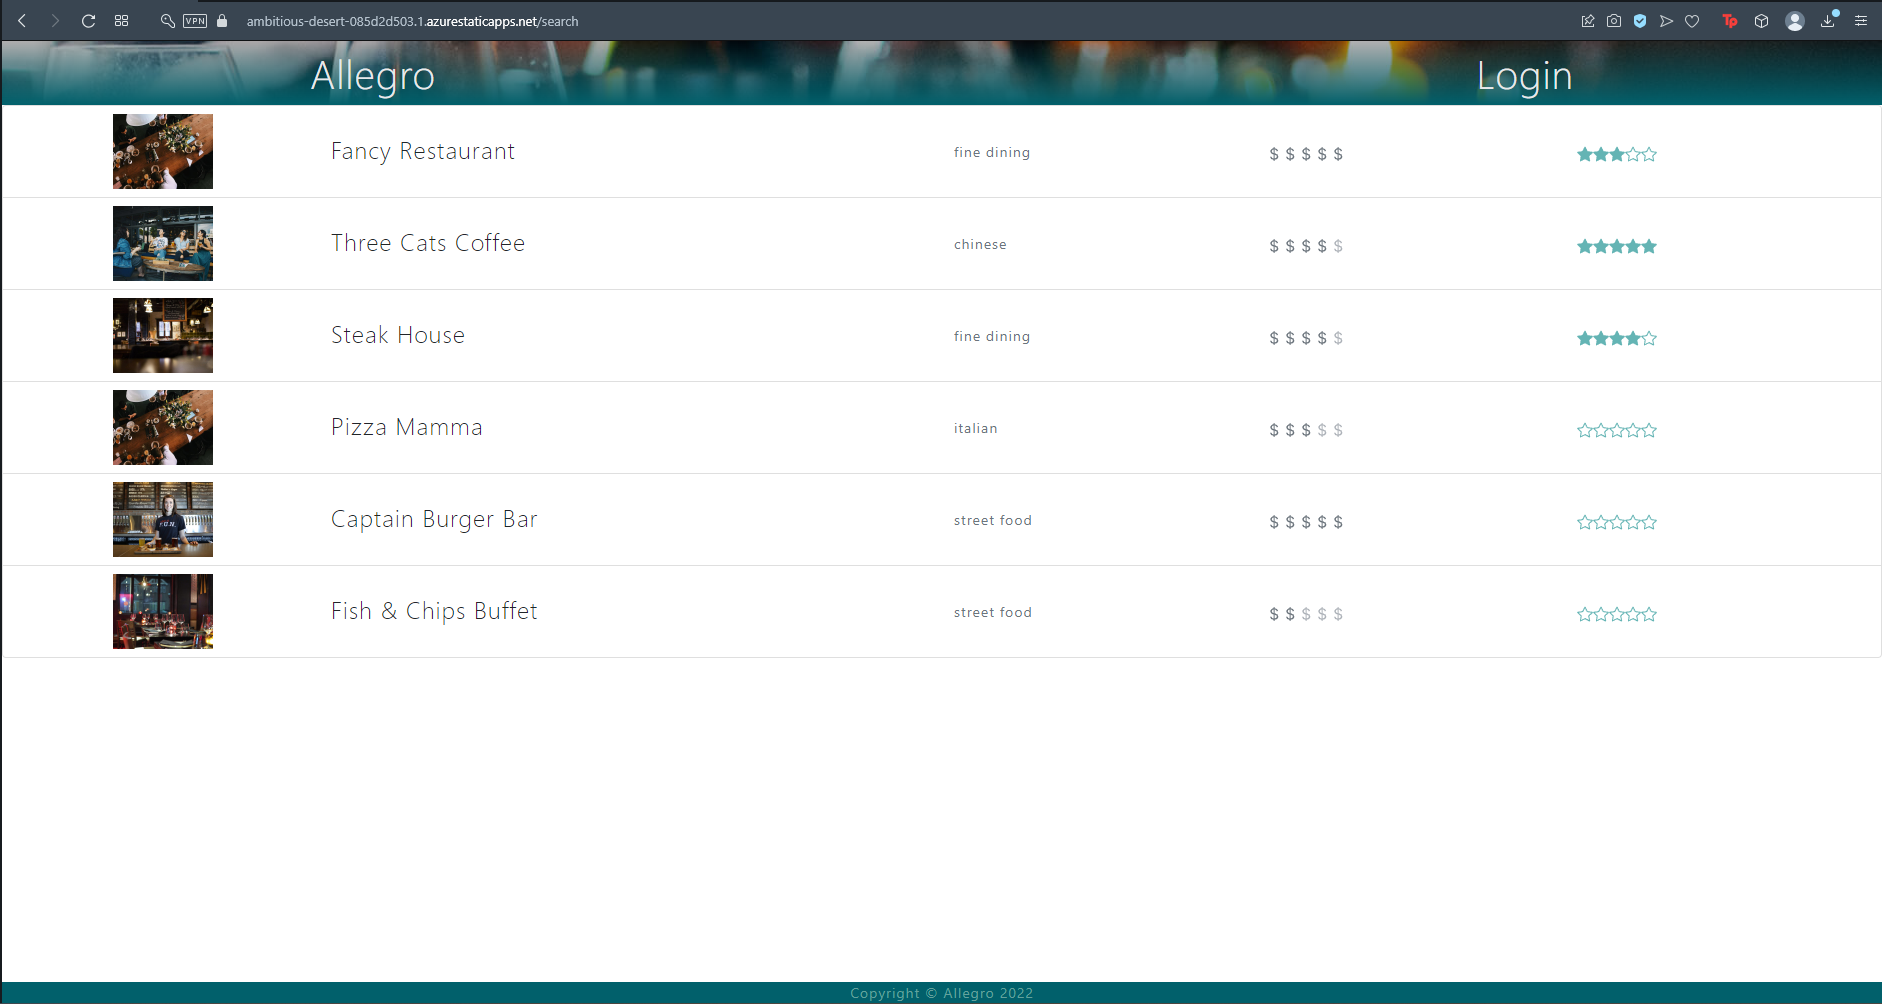
\includegraphics[width=150mm, keepaspectratio]{figures/UI/1_RestaurantList.png}
	\caption{Restaurant list component UI} 
	\label{fig:UI_1}
\end{figure}

\begin{figure}[ht]
	\centering
	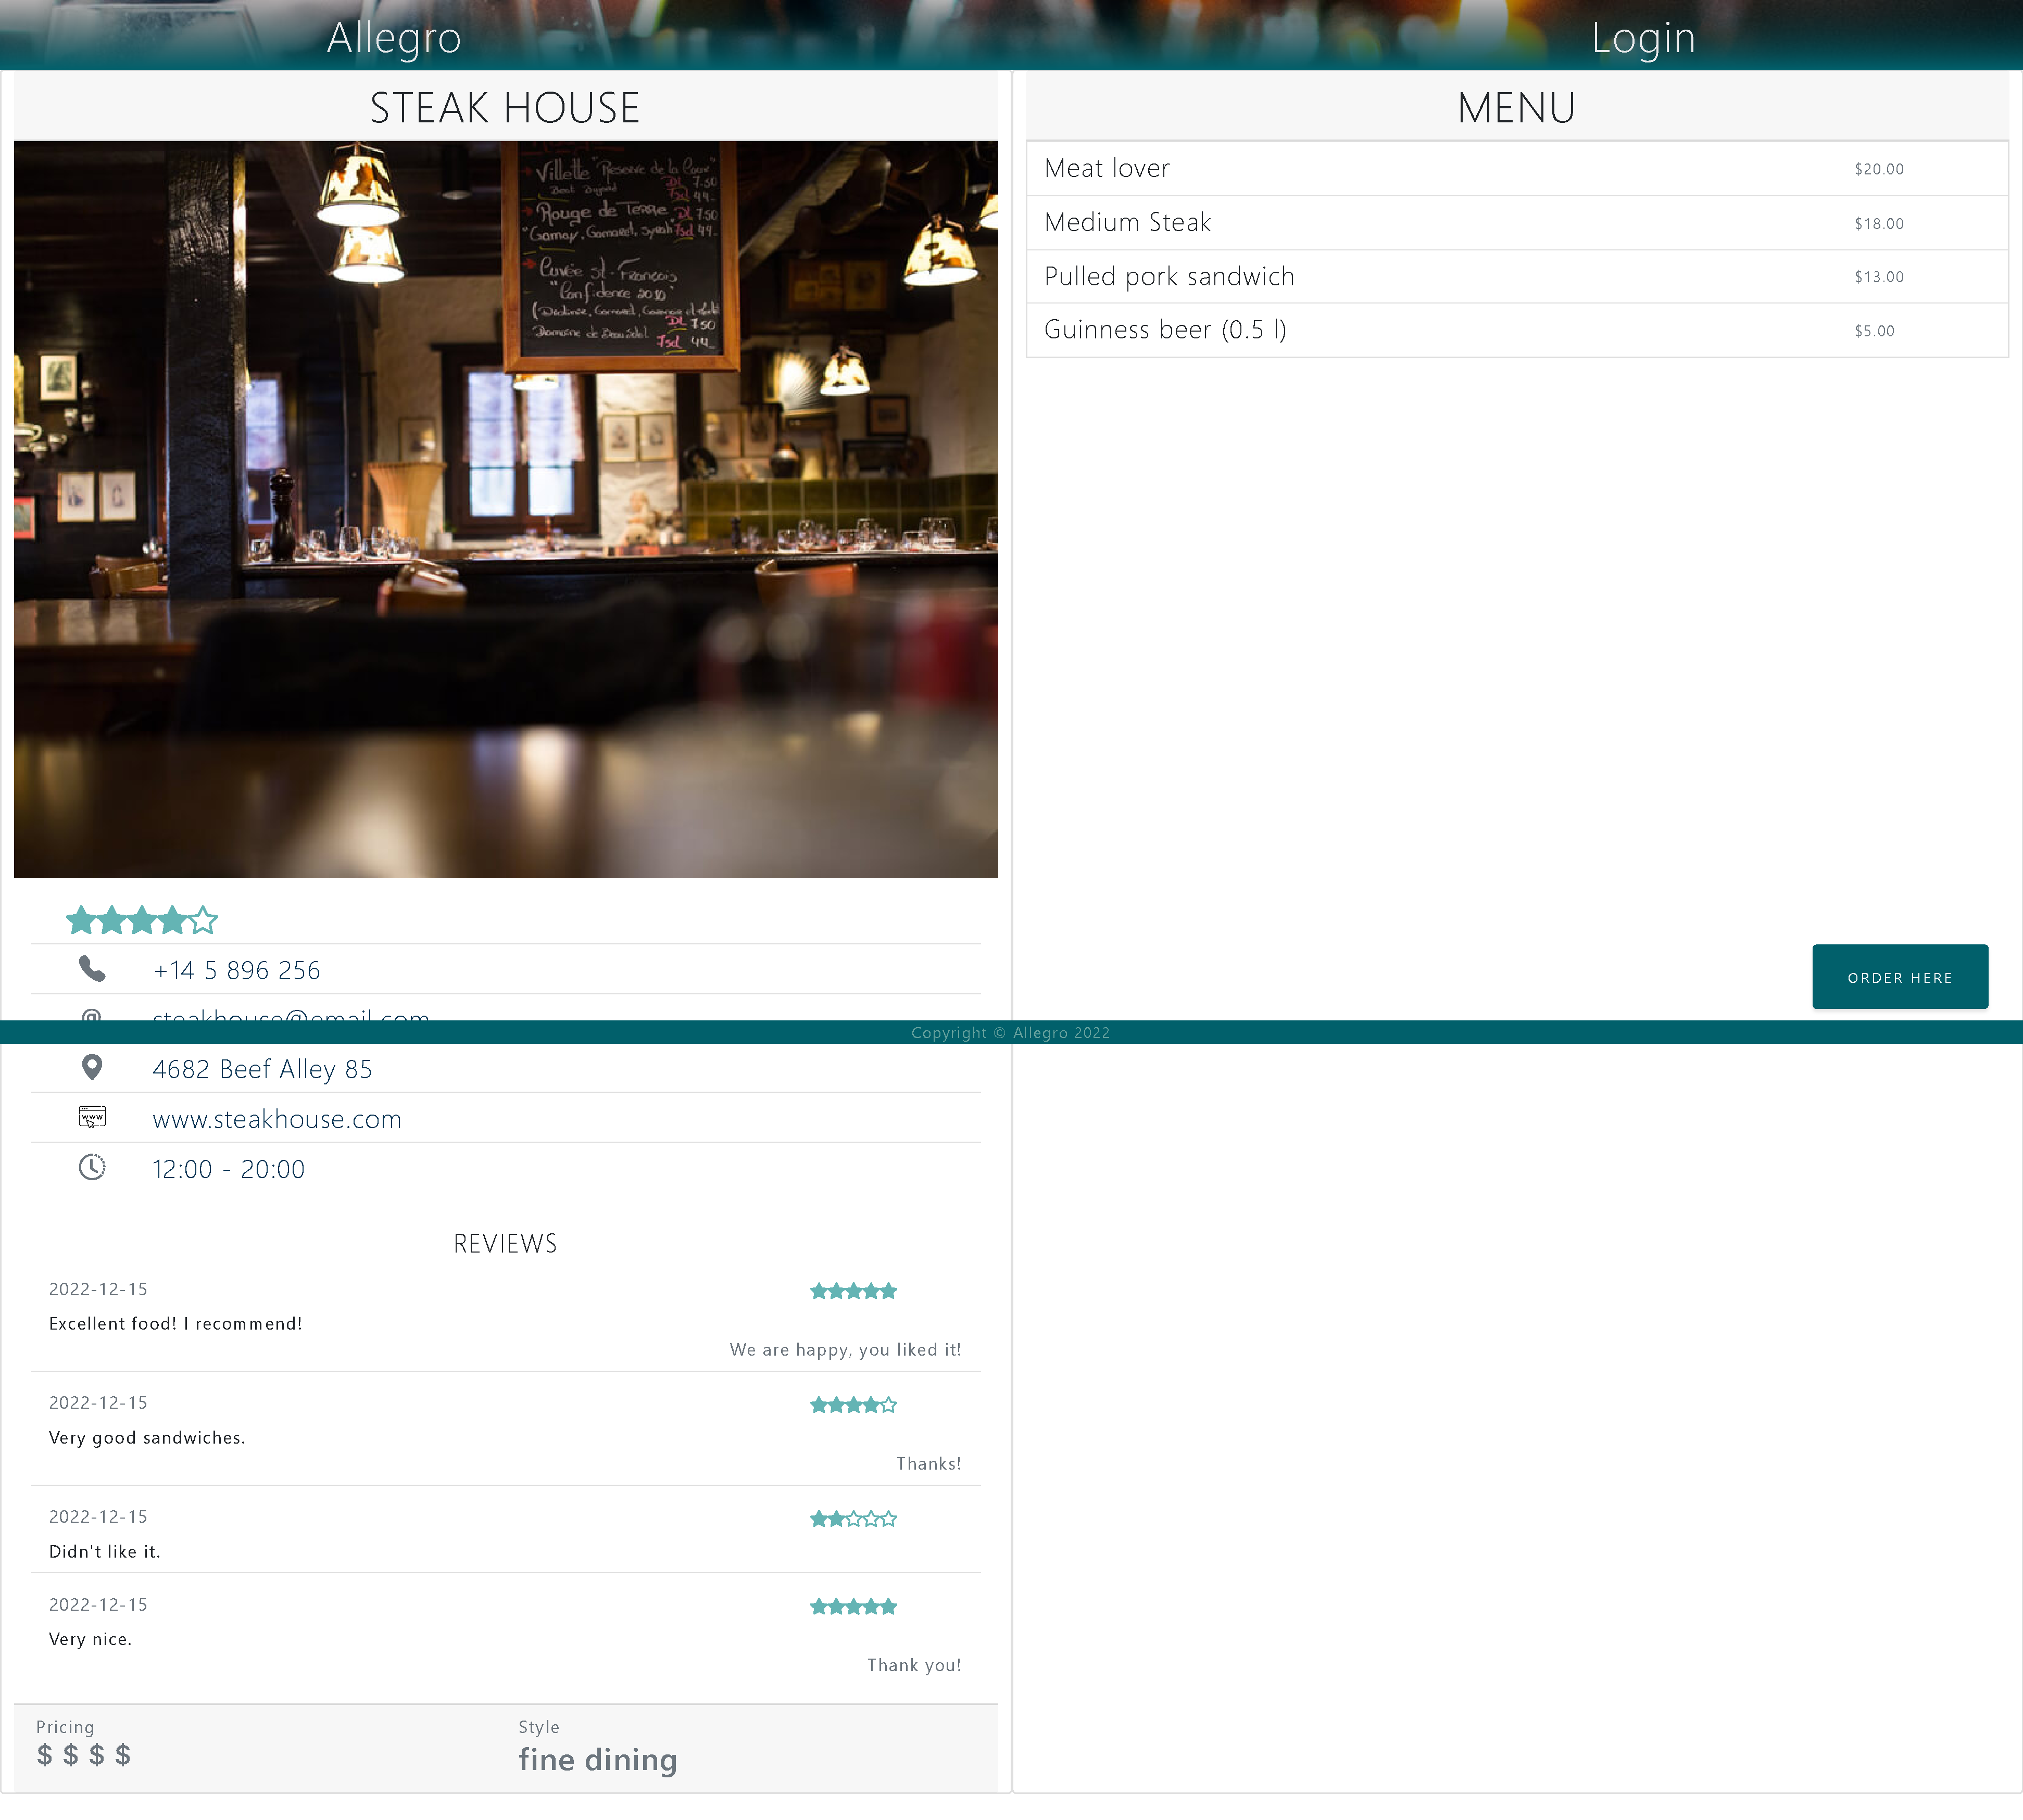
\includegraphics[width=150mm, keepaspectratio]{figures/UI/2_RestaurantDetails}
	\caption{Restaurant details component UI} 
	\label{fig:UI_2}
\end{figure}

\begin{figure}[ht]
	\centering
	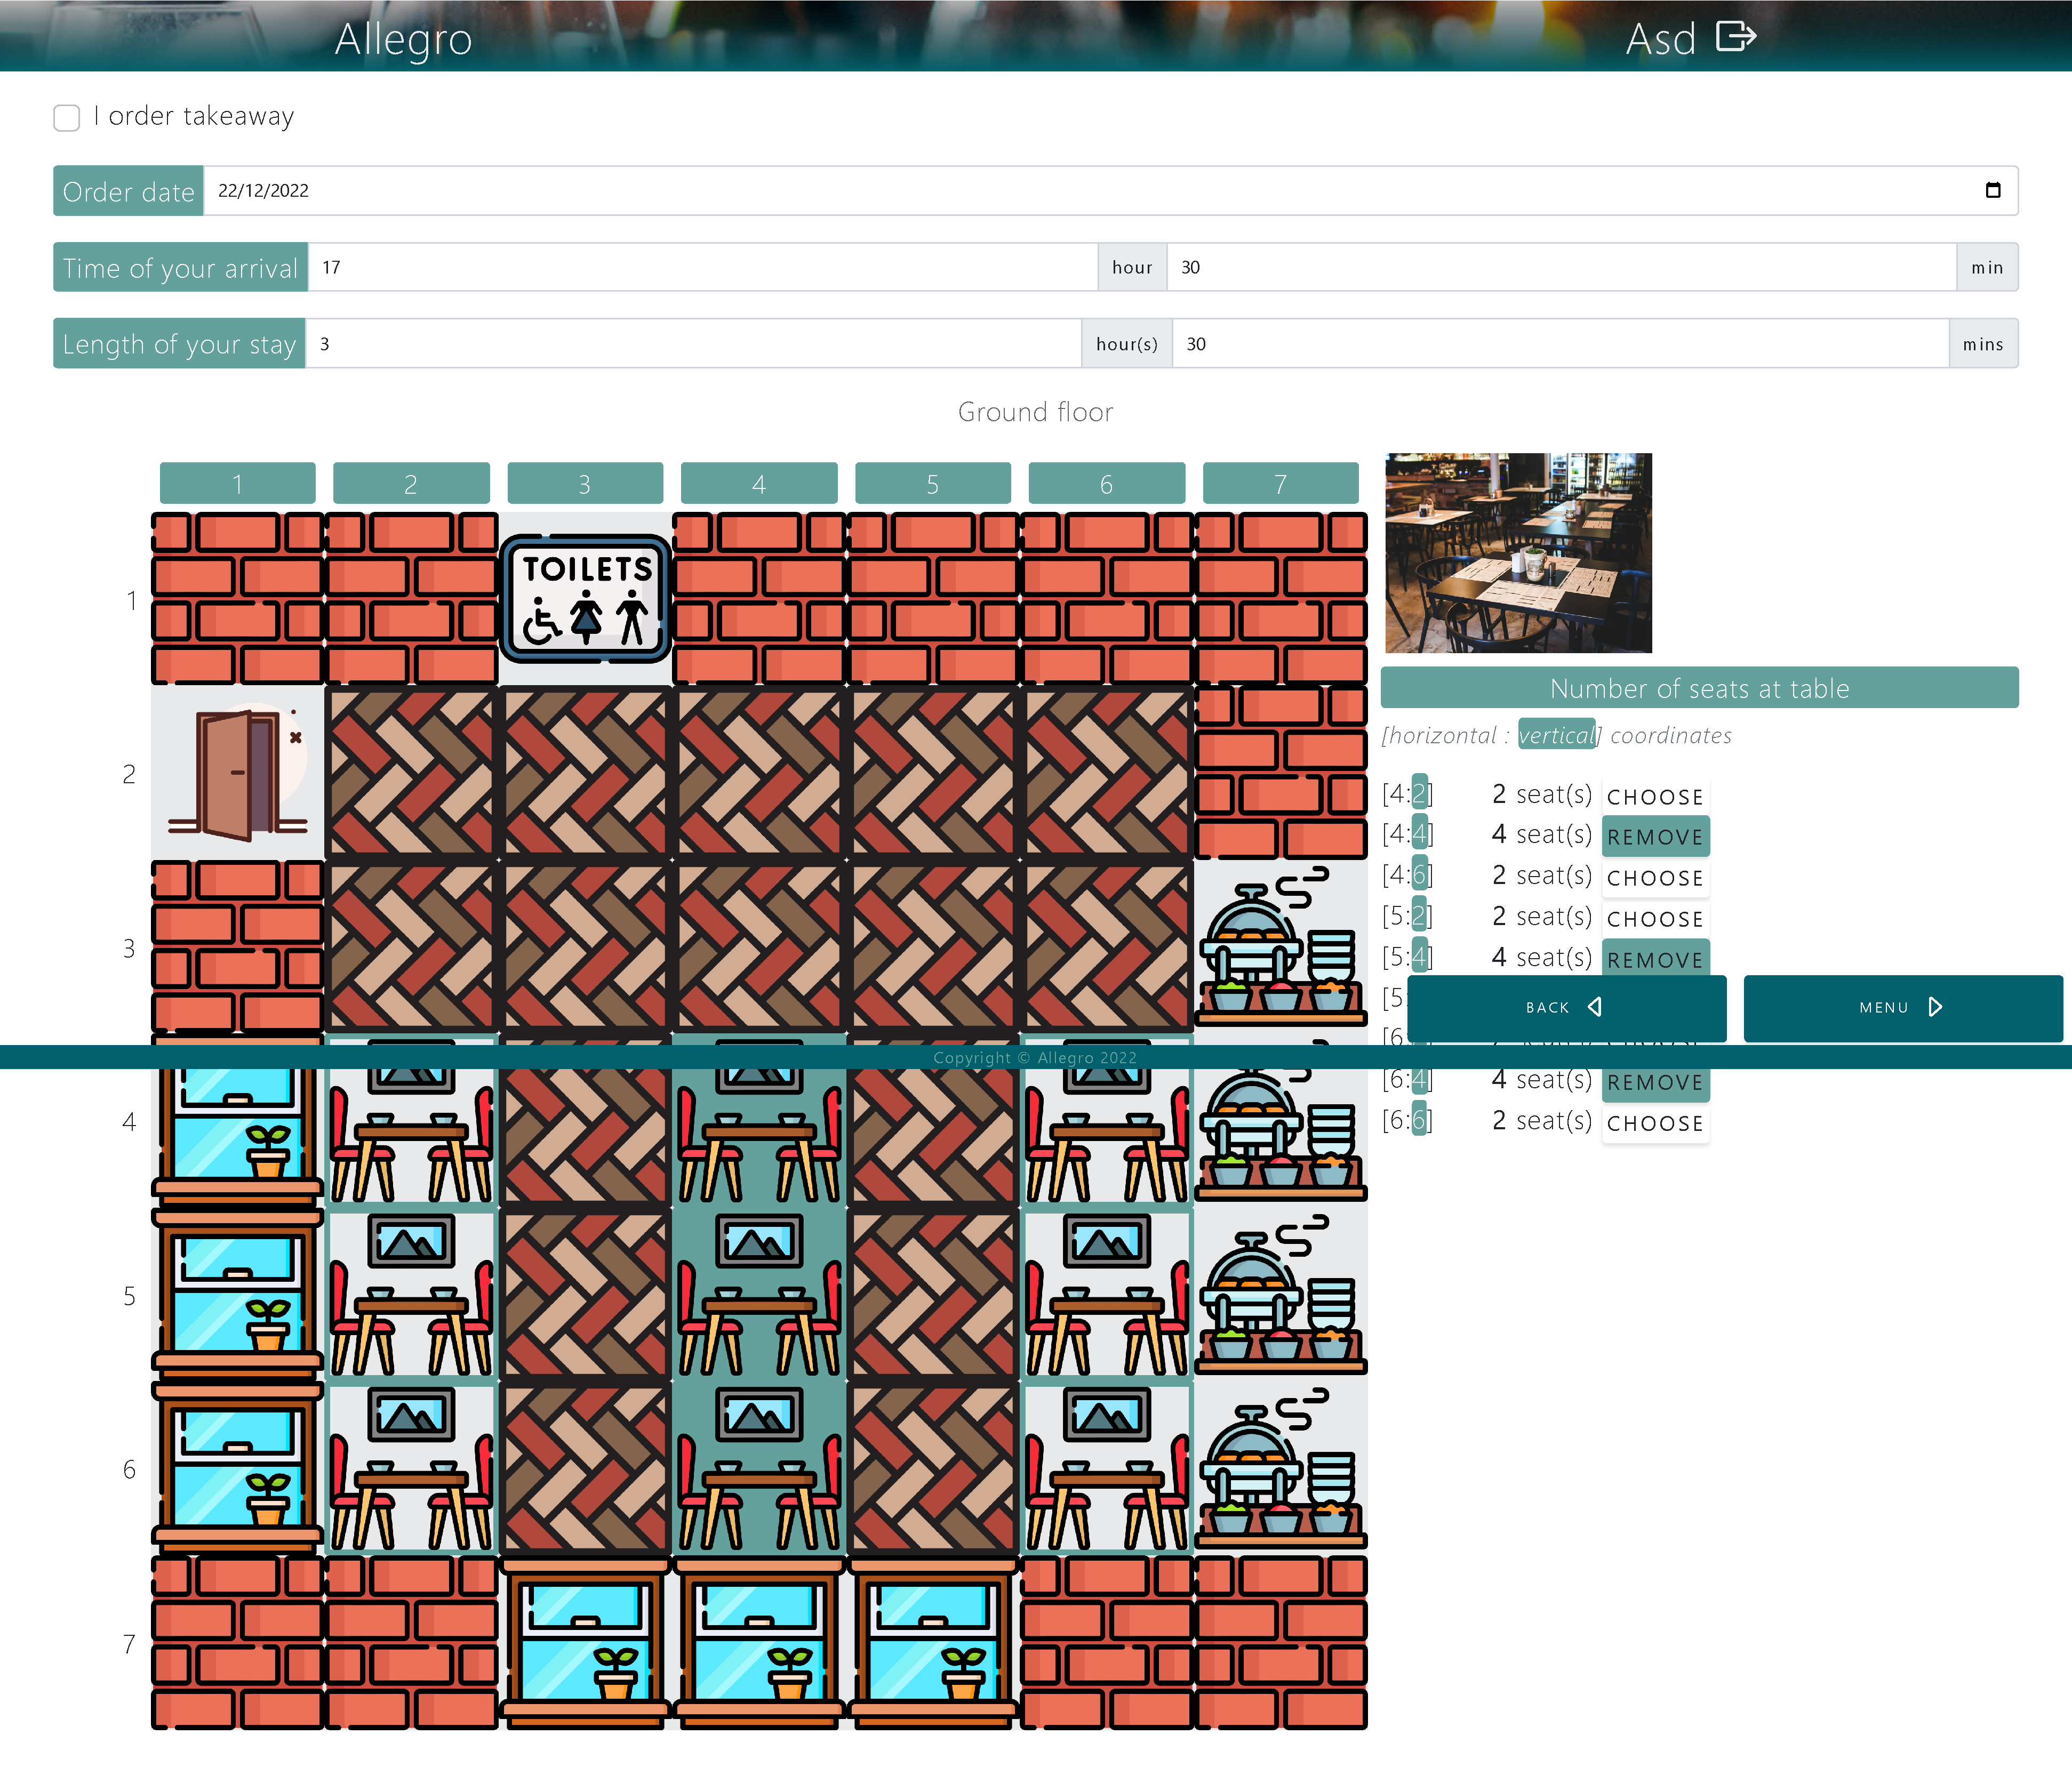
\includegraphics[width=150mm, keepaspectratio]{figures/UI/4_Reservation}
	\caption{Reservation component UI} 
	\label{fig:UI_4}
\end{figure}

\begin{figure}[ht]
	\centering
	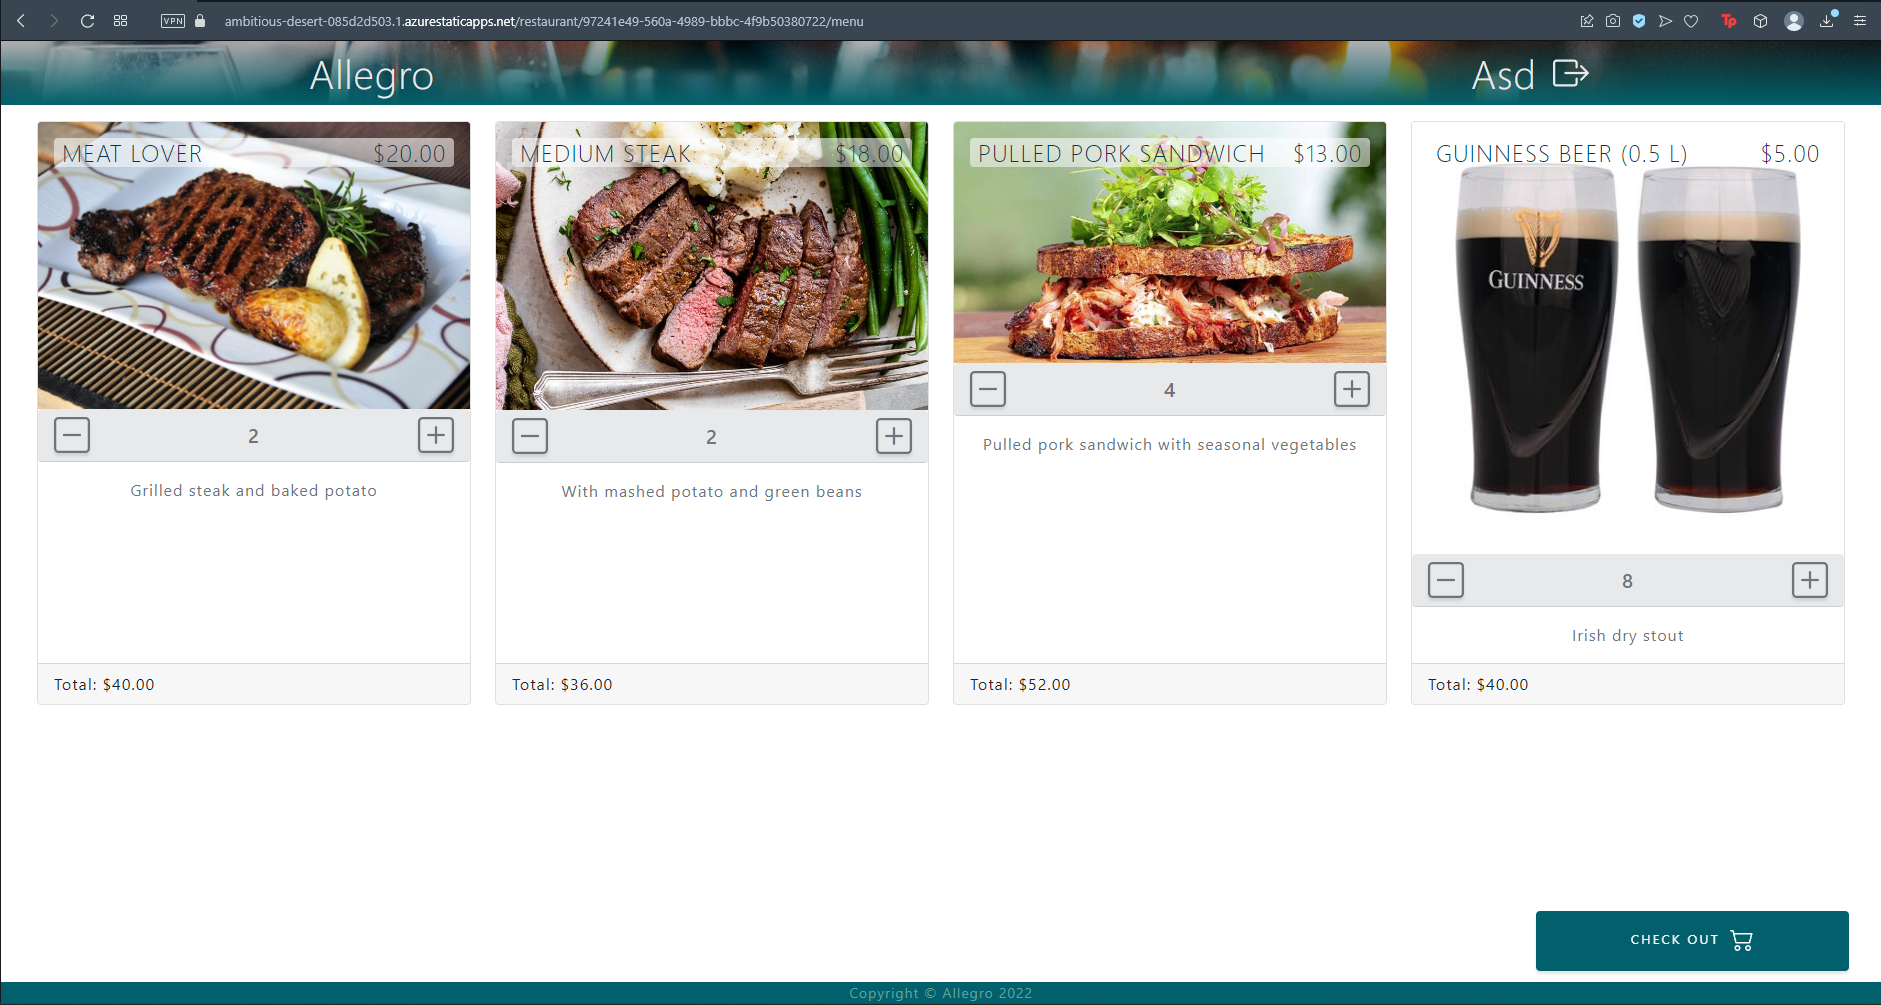
\includegraphics[width=150mm, keepaspectratio]{figures/UI/5_Order.png}
	\caption{Order component UI} 
	\label{fig:UI_5}
\end{figure}

\begin{figure}[ht]
\centering
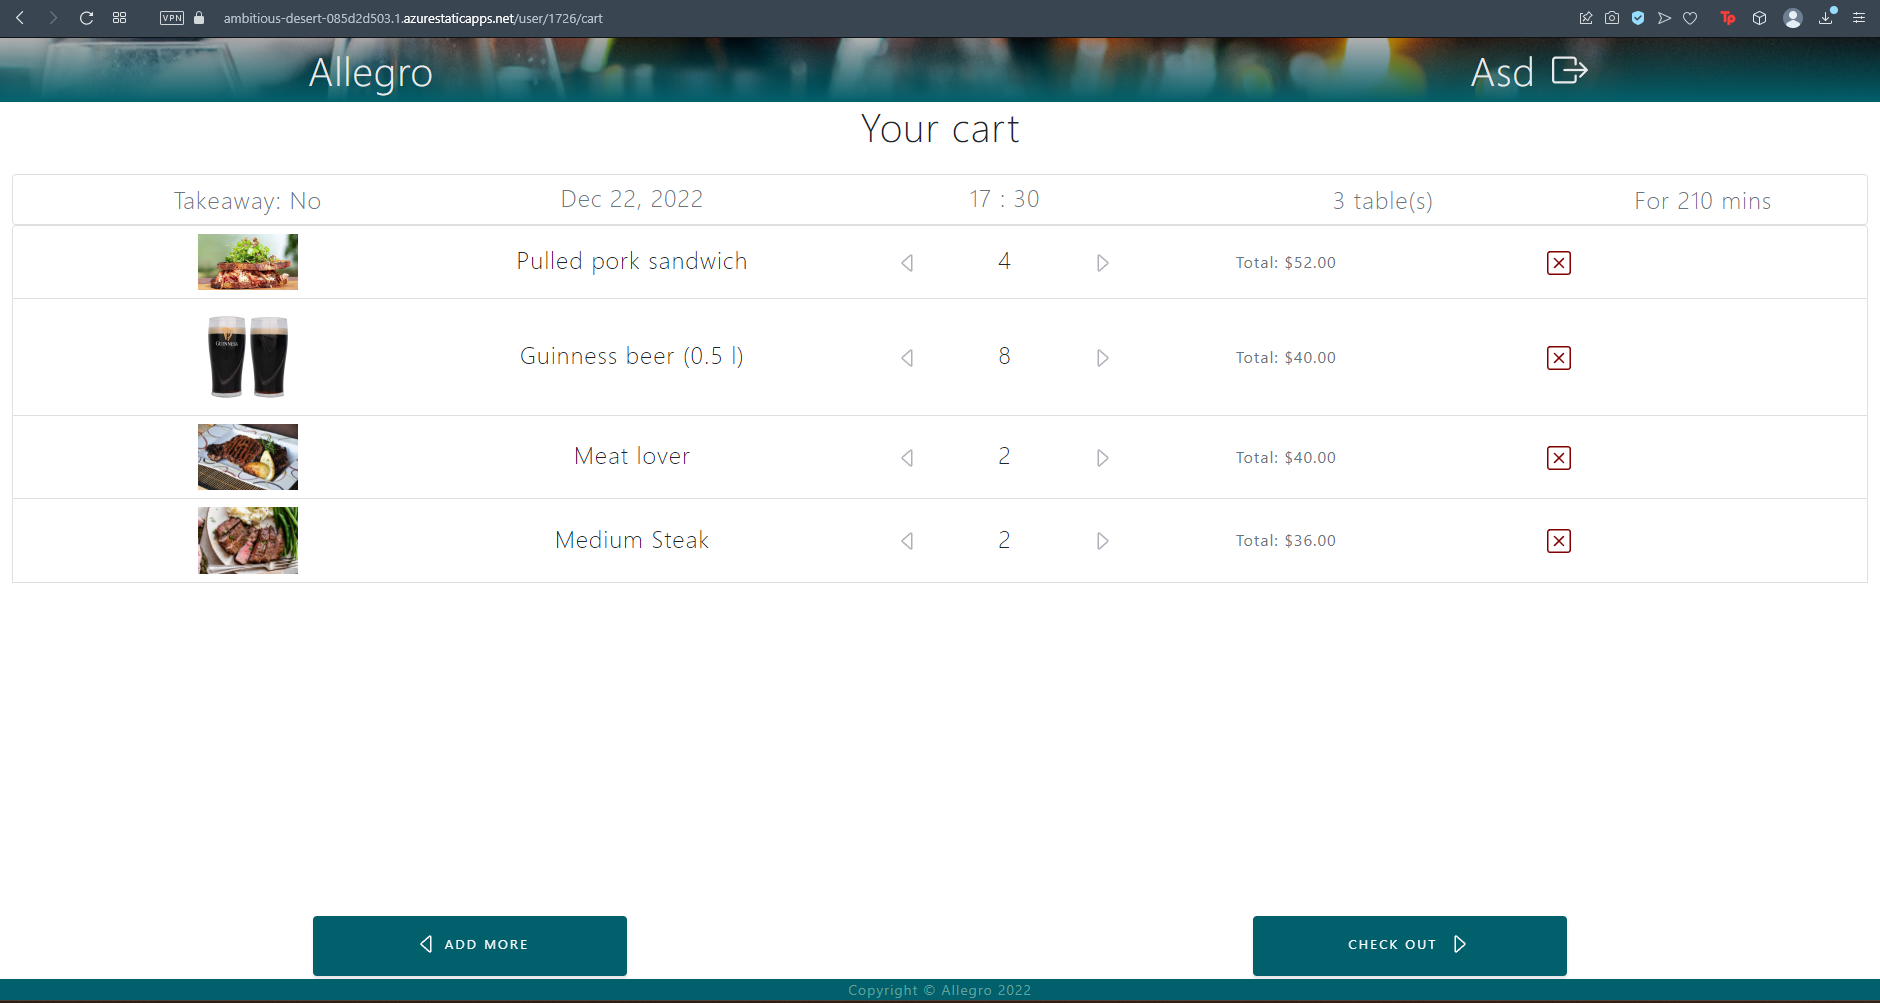
\includegraphics[width=150mm, keepaspectratio]{figures/UI/3_Cart.png}
\caption{Cart component UI} 
\label{fig:UI_3}
\end{figure}

\begin{figure}[ht]
	\centering
	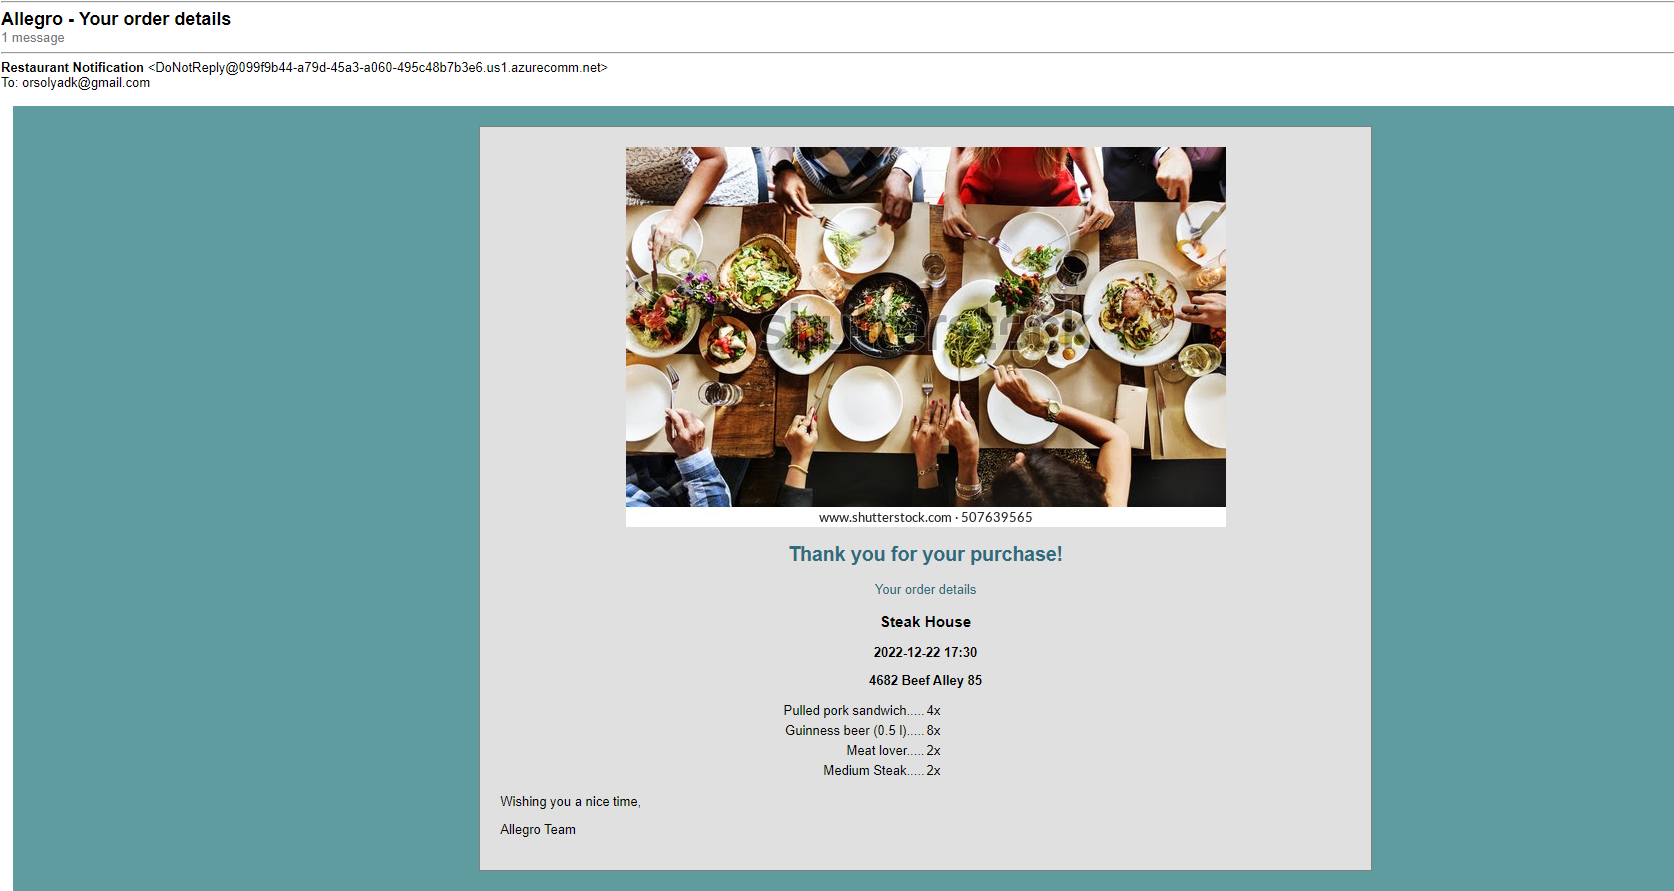
\includegraphics[width=150mm, keepaspectratio]{figures/UI/7_Email_1.png}
	\caption{Sent e-mails} 
	\label{fig:UI_6}
\end{figure}

\begin{figure}[ht]
	\centering
	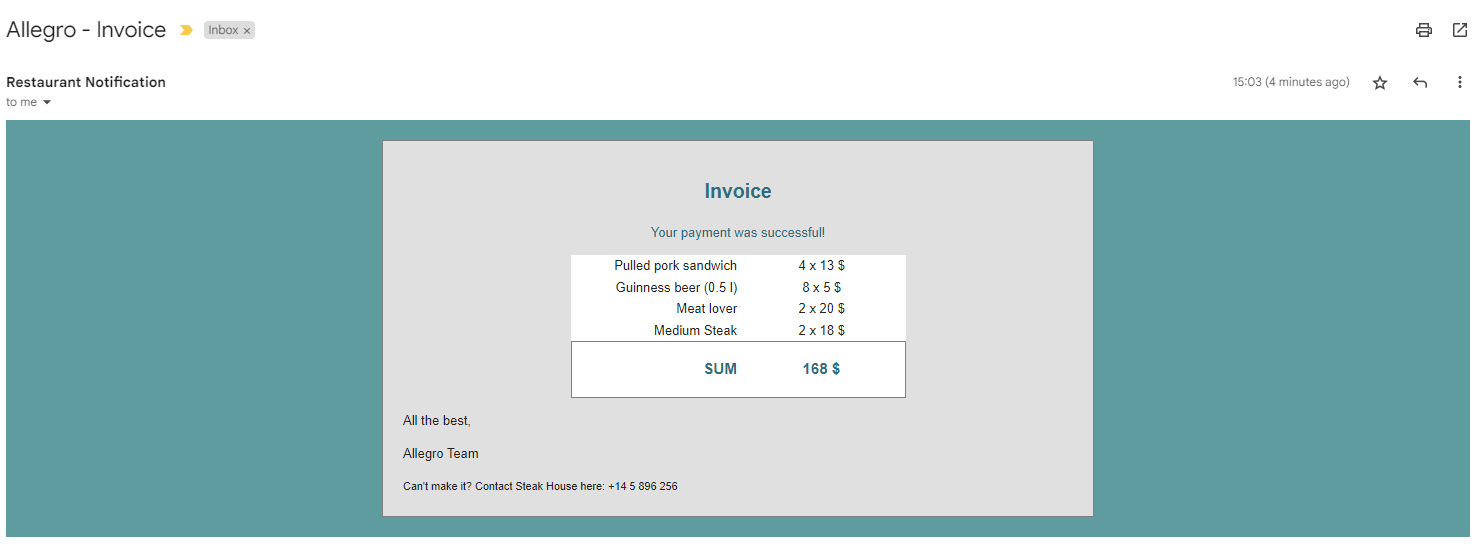
\includegraphics[width=150mm, keepaspectratio]{figures/UI/7_Email_2.png}
	\caption{Sent e-mails} 
	\label{fig:UI_7}
\end{figure}

\begin{figure}[ht]
	\centering
	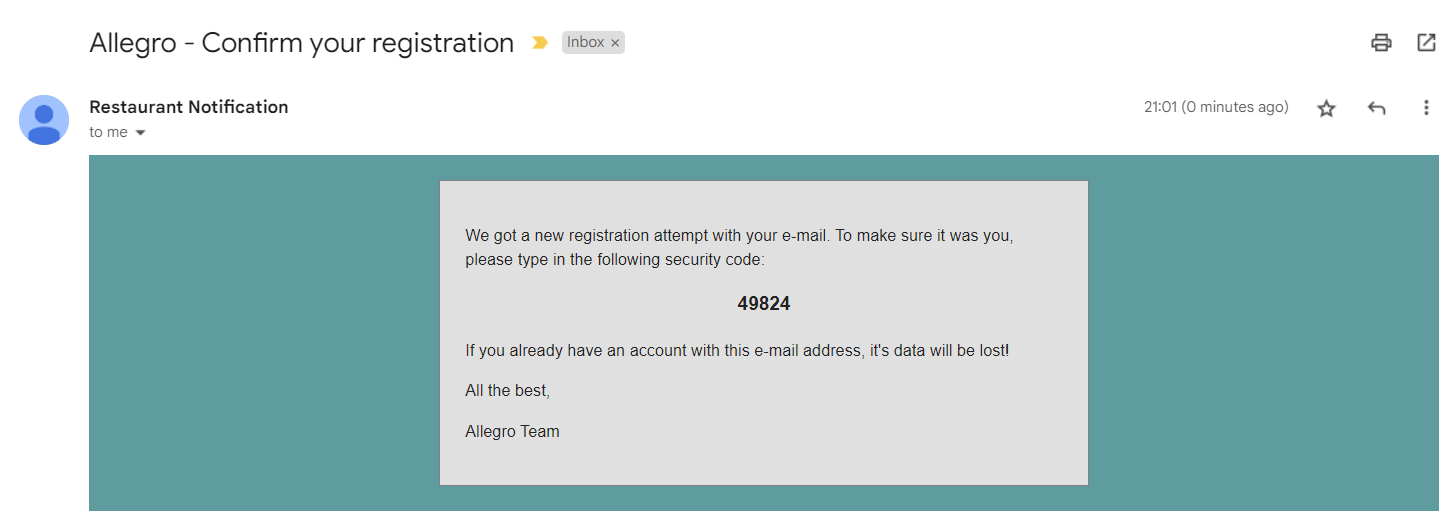
\includegraphics[width=150mm, keepaspectratio]{figures/UI/7_Email_3.png}
	\caption{Sent e-mails} 
	\label{fig:UI_7.1}
\end{figure}

\begin{figure}[ht]
	\centering
	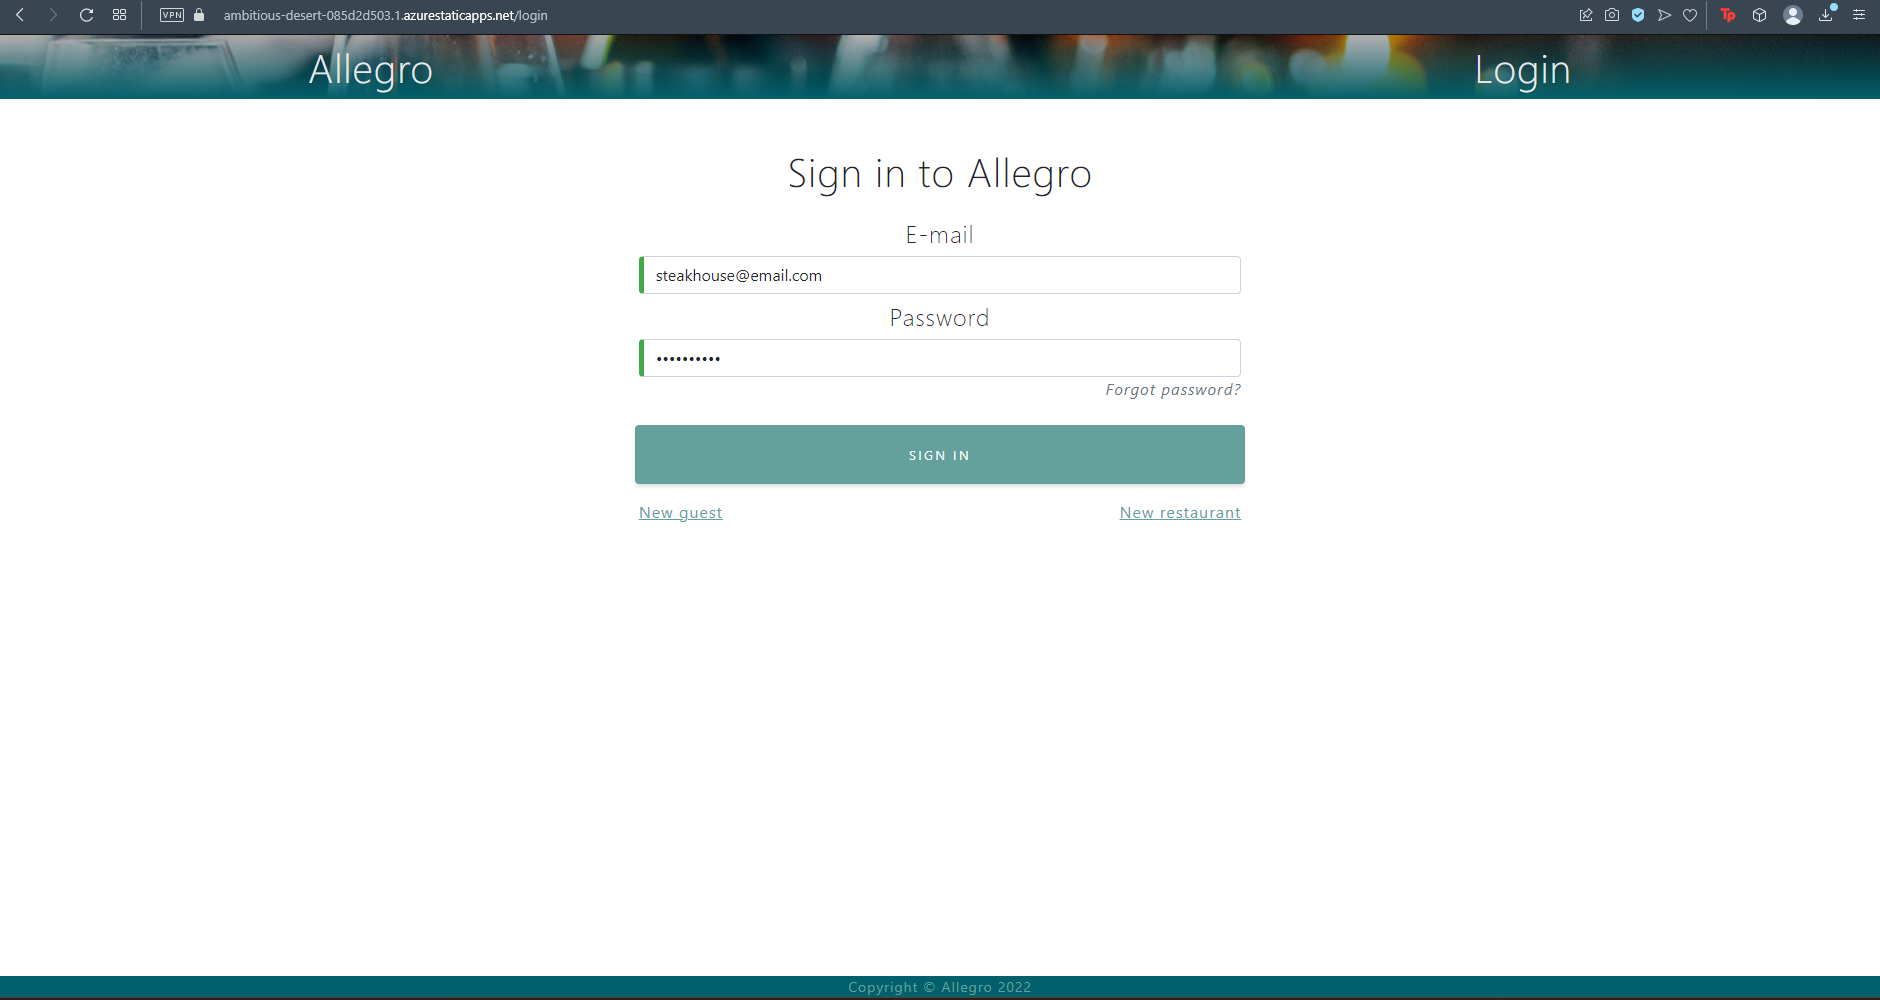
\includegraphics[width=150mm, keepaspectratio]{figures/UI/8_Login.png}
	\caption{Login component UI} 
	\label{fig:UI_8}
\end{figure}

\begin{figure}[ht]
	\centering
	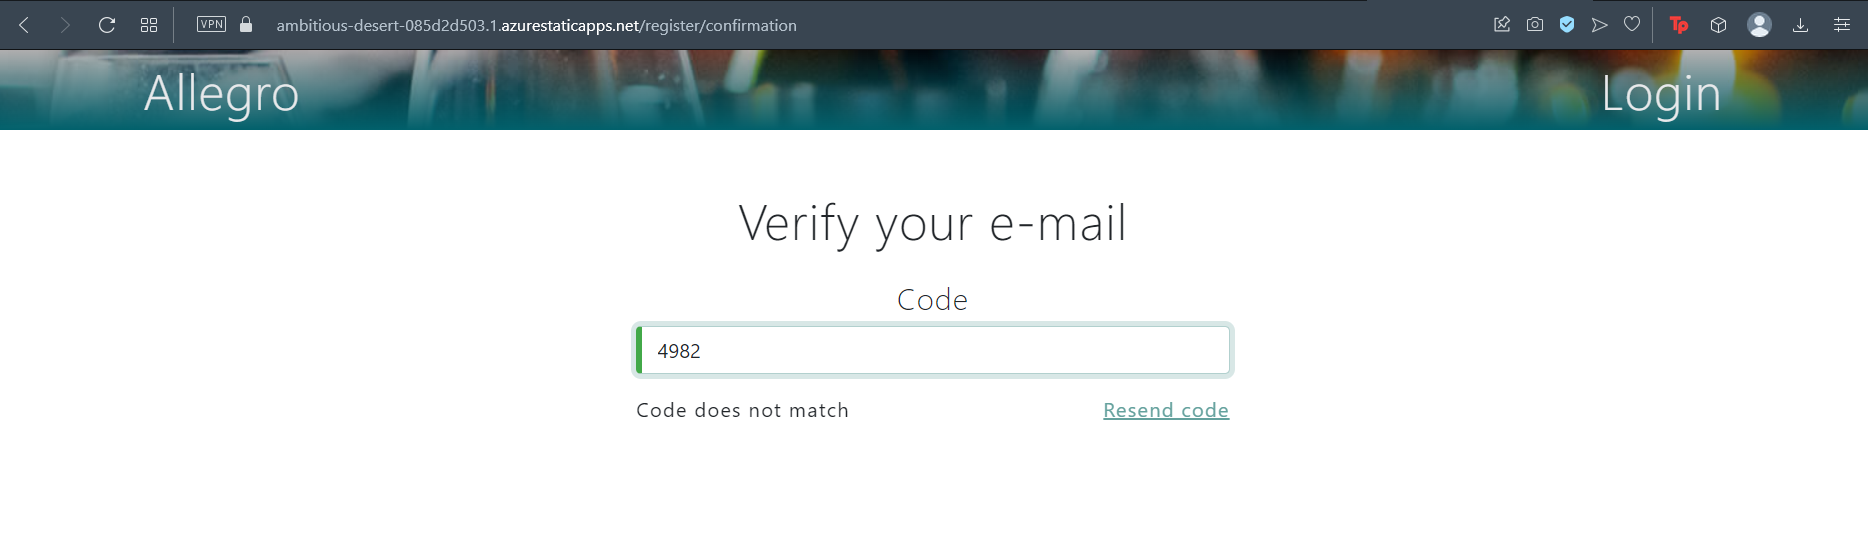
\includegraphics[width=150mm, keepaspectratio]{figures/UI/8_ConfirmFalse.png}
	\caption{Wrong confirmation code} 
	\label{fig:UI_8.2}
\end{figure}

\begin{figure}[ht]
	\centering
	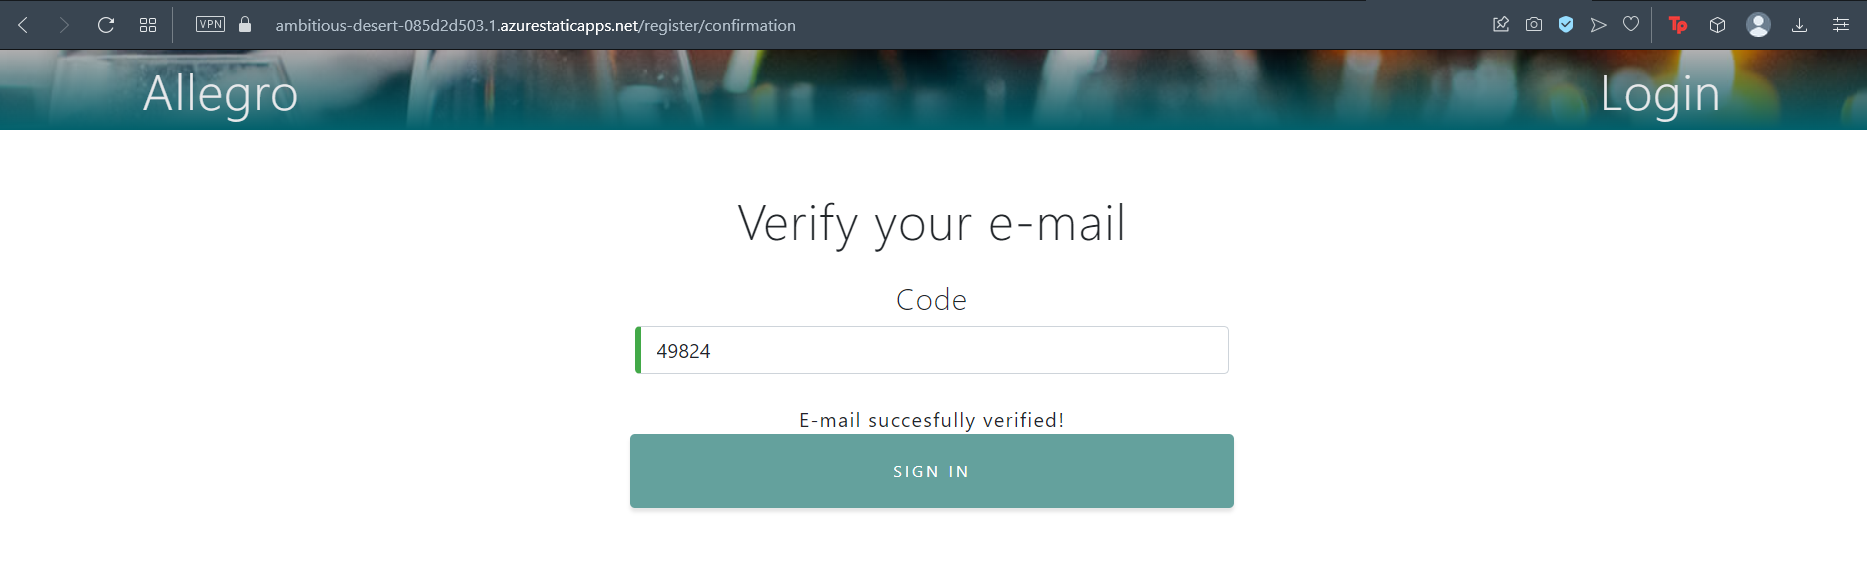
\includegraphics[width=150mm, keepaspectratio]{figures/UI/8_ConfirmSuccess.png}
	\caption{Successful confirmation} 
	\label{fig:UI_8.3}
\end{figure}

\begin{figure}[ht]
	\centering
	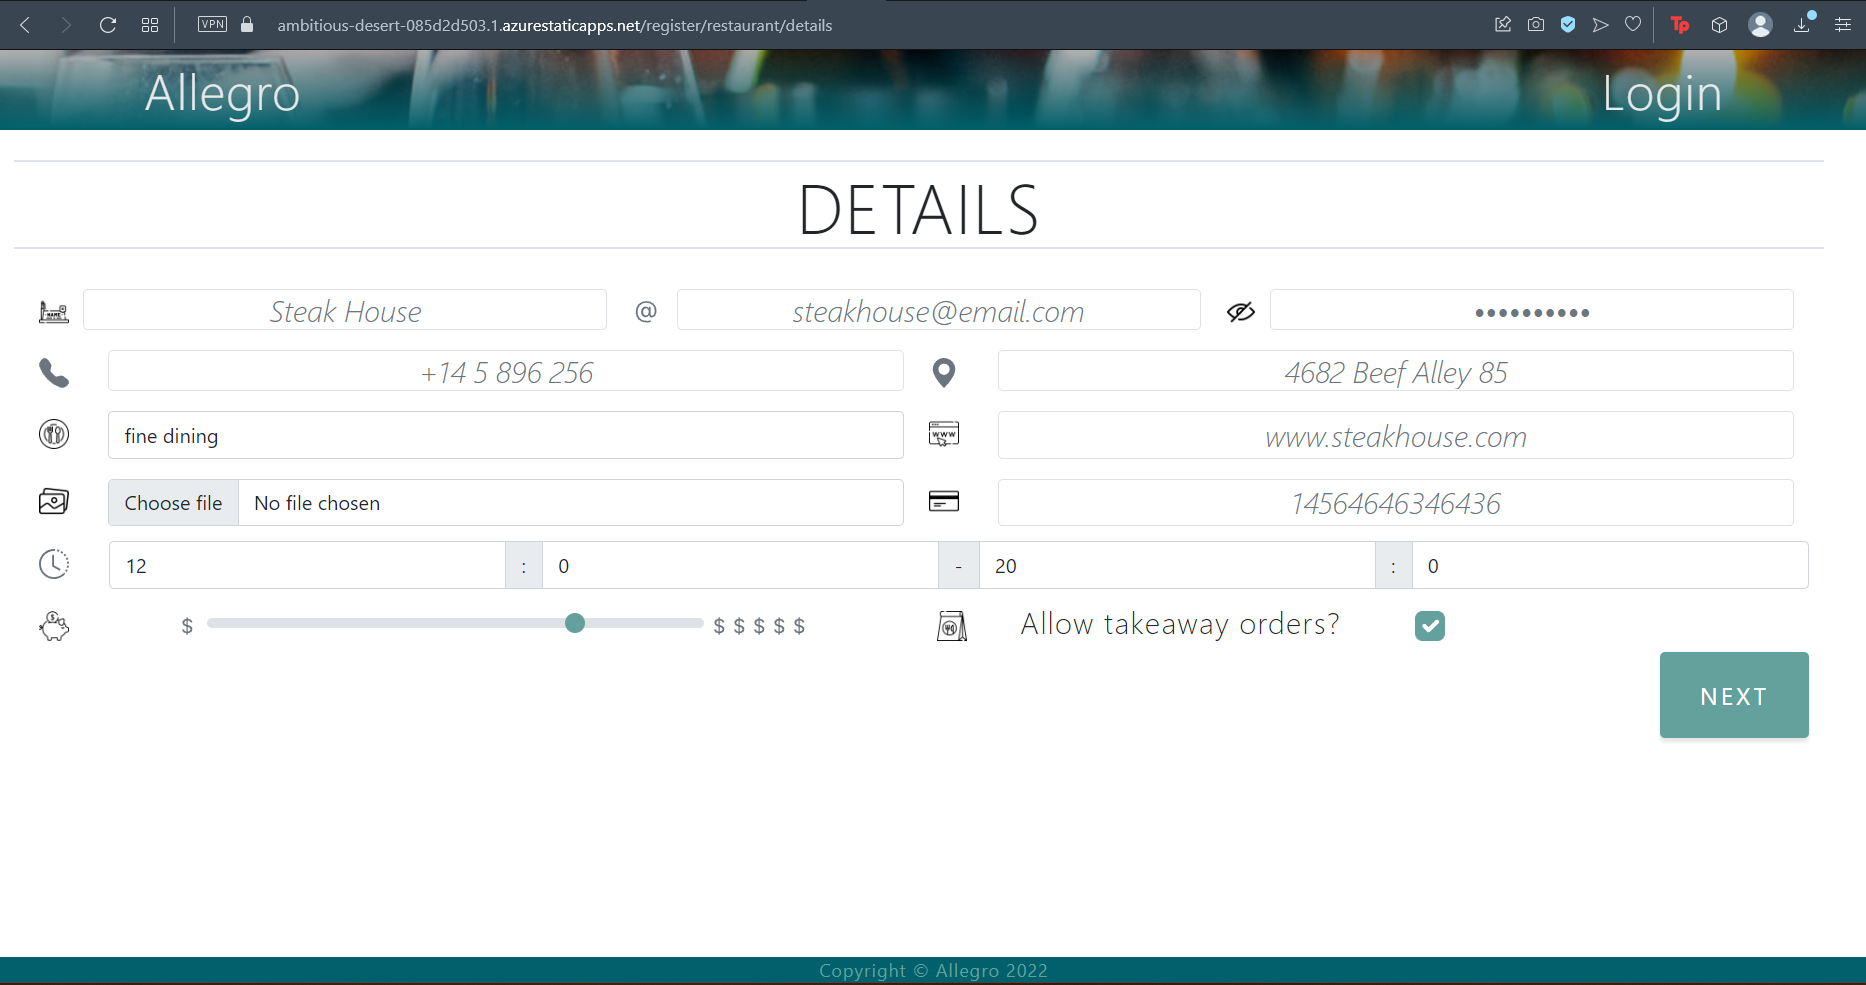
\includegraphics[width=150mm, keepaspectratio]{figures/UI/9_RestaurantDetailsEdit.png}
	\caption{Restaurant details registration UI} 
	\label{fig:UI_9}
\end{figure}

\begin{figure}[ht]
	\centering
	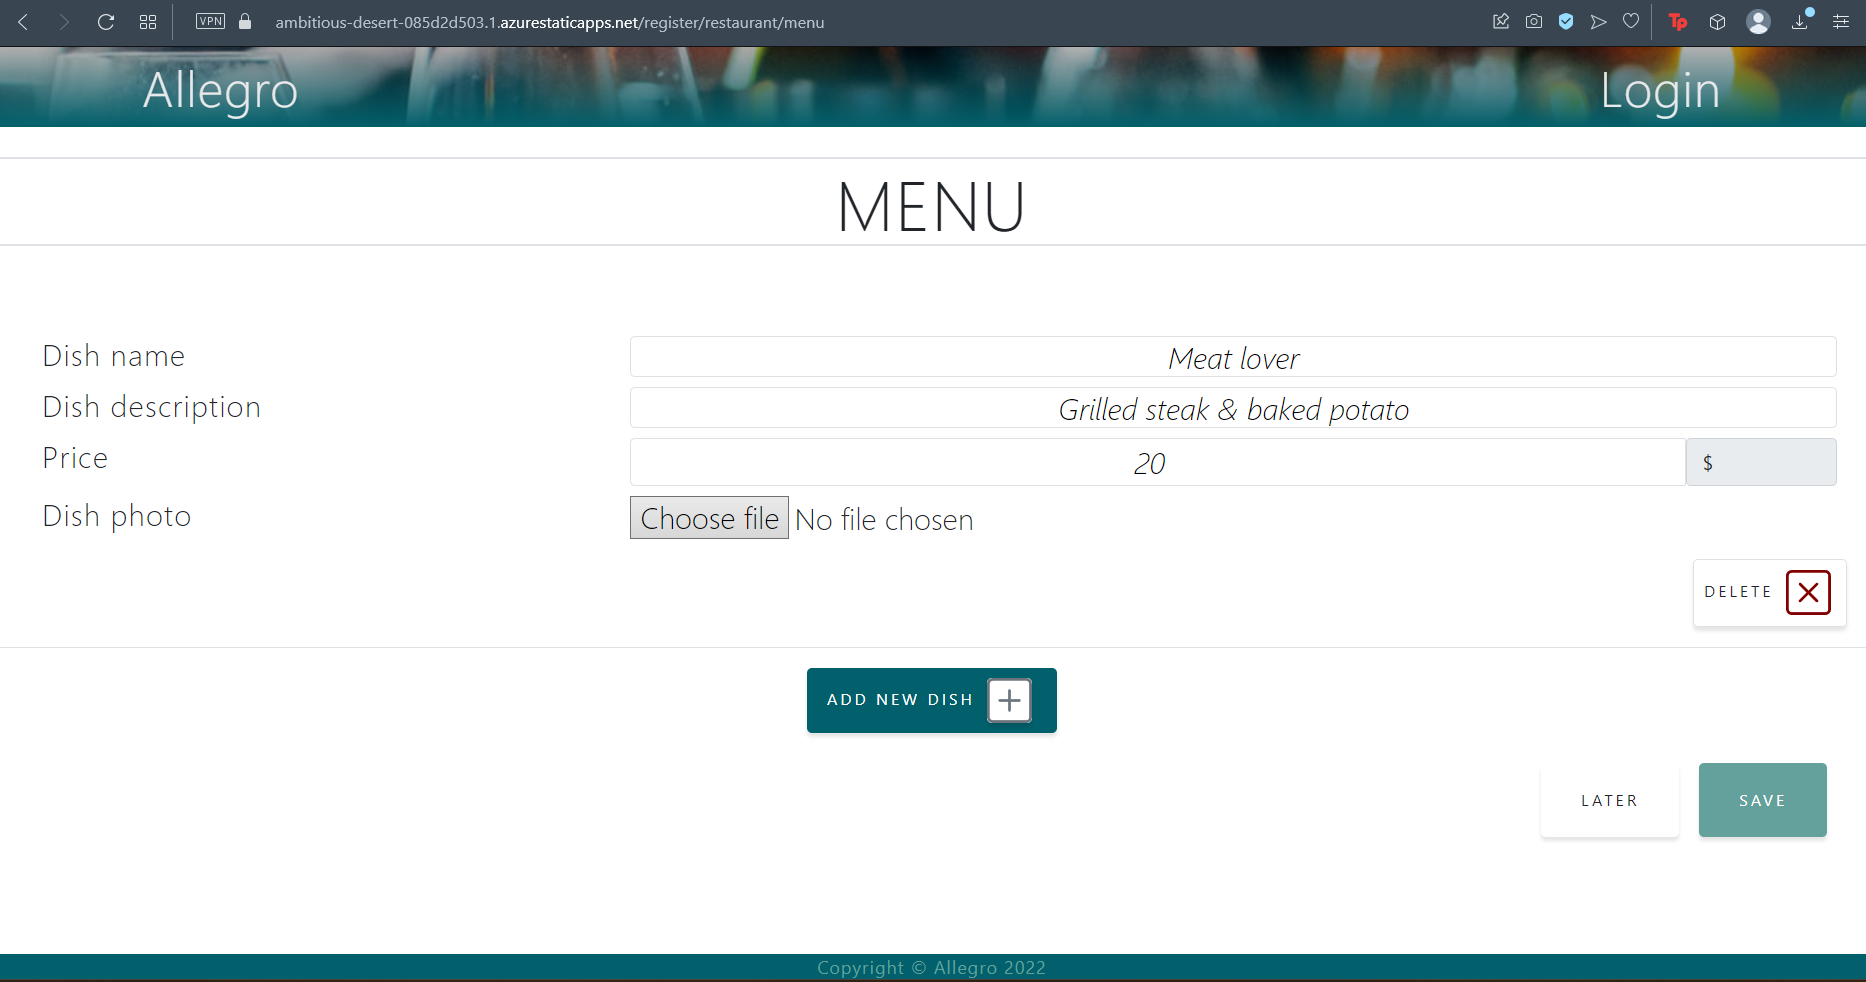
\includegraphics[width=150mm, keepaspectratio]{figures/UI/10_RestaurantMenuEdit.png}
	\caption{Restaurant menu registration UI} 
	\label{fig:UI_10}
\end{figure}

\begin{figure}[ht]
	\centering
	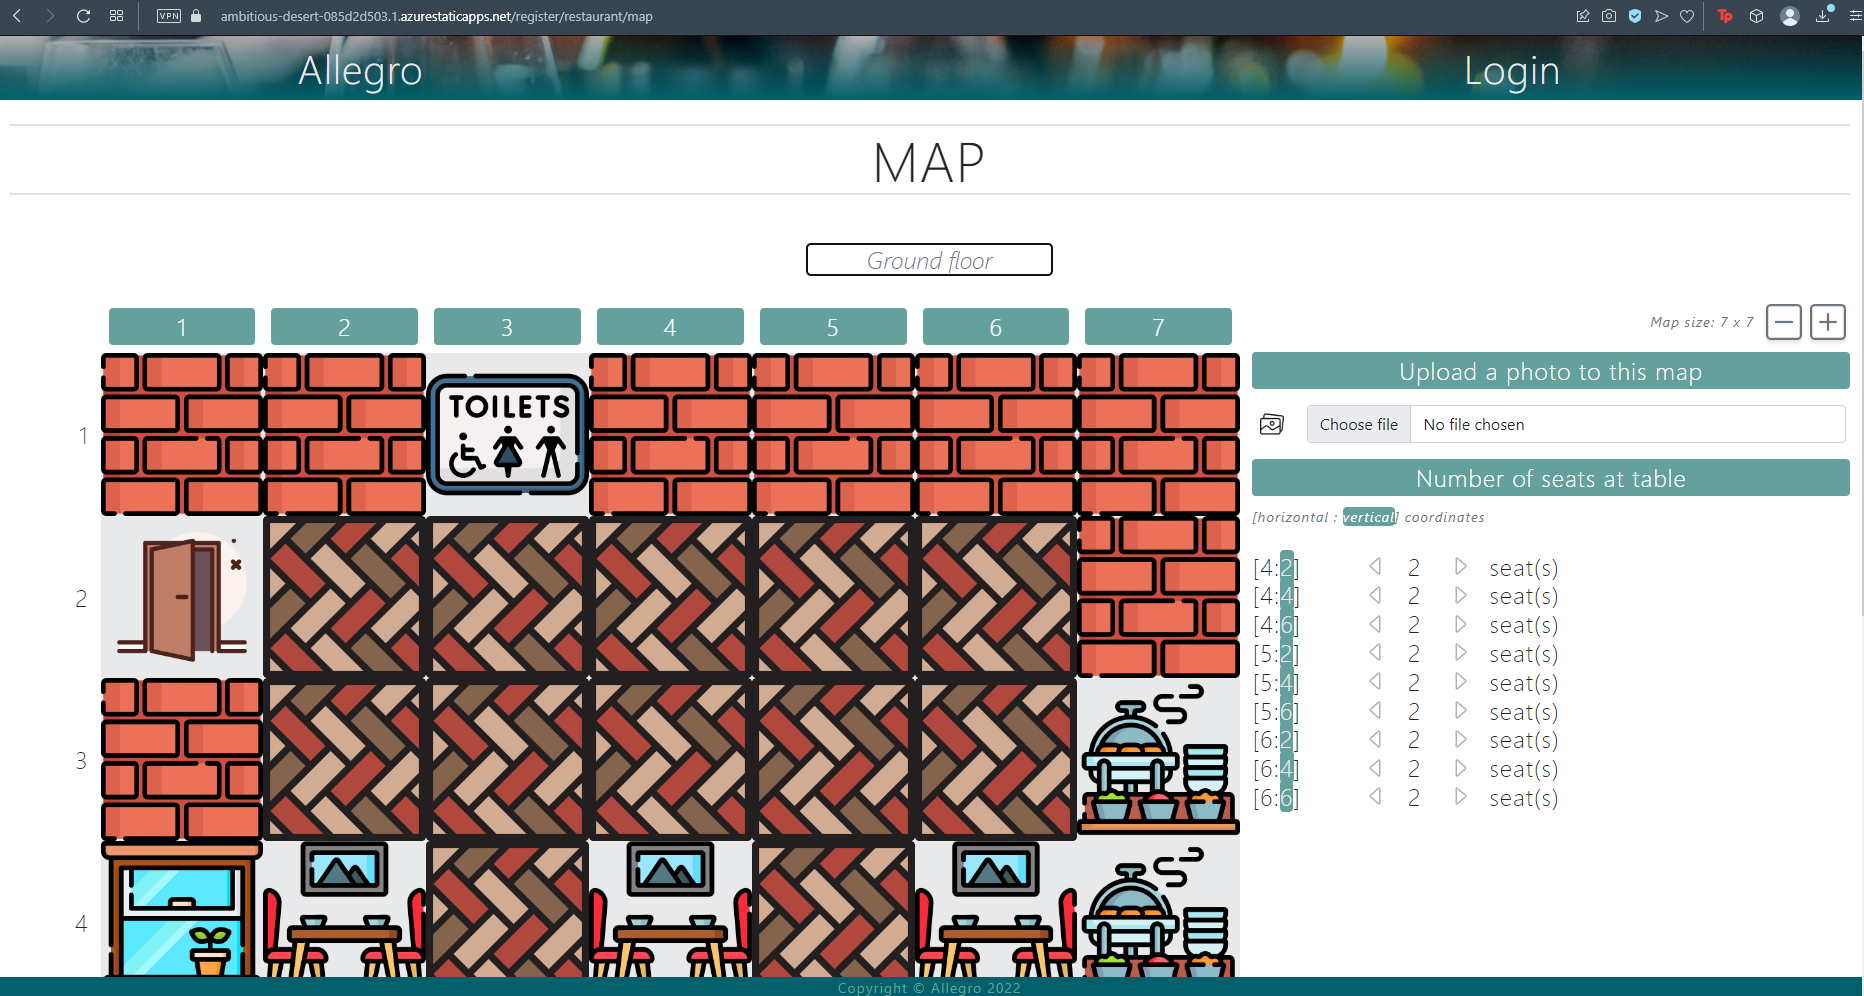
\includegraphics[width=150mm, keepaspectratio]{figures/UI/11_RestaurantMapEdit.png}
	\caption{Restaurant map registration UI} 
	\label{fig:UI_11}
\end{figure}

\begin{figure}[ht]
	\centering
	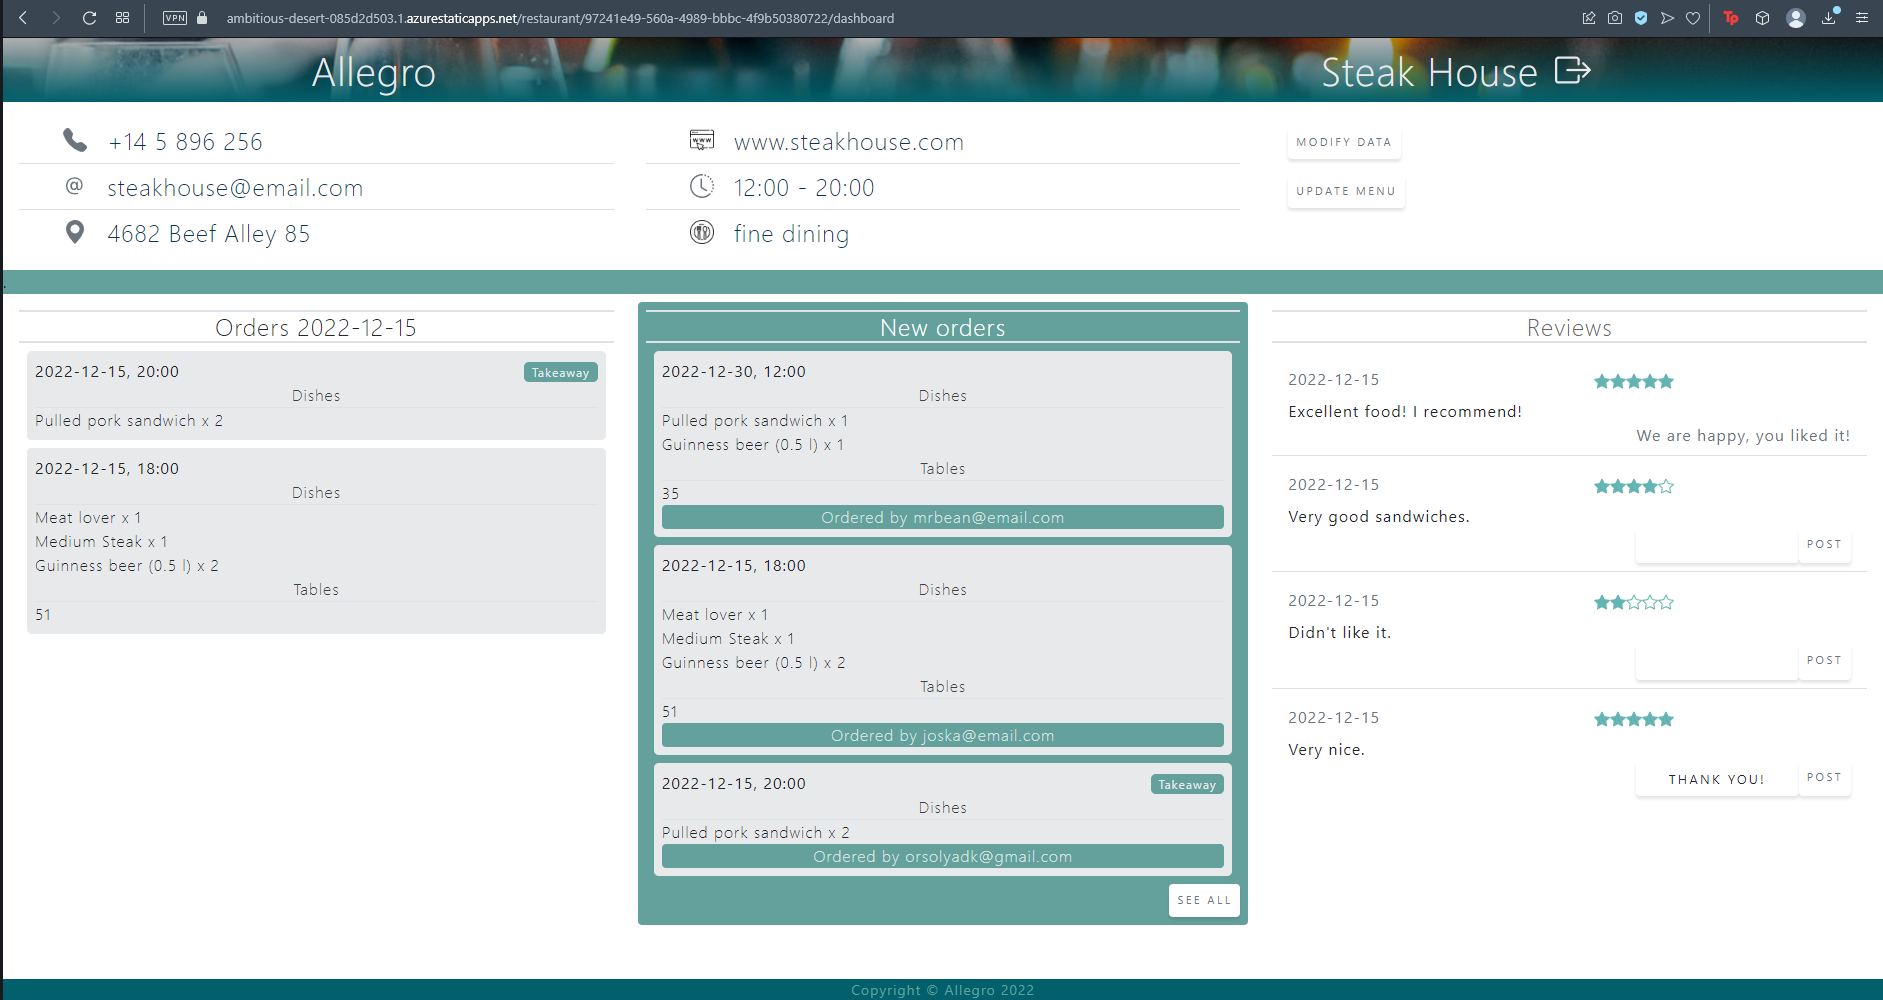
\includegraphics[width=150mm, keepaspectratio]{figures/UI/12_Dashboard.png}
	\caption{Restaurant dashboard UI} 
	\label{fig:UI_12}
\end{figure}

\begin{figure}[ht]
	\centering
	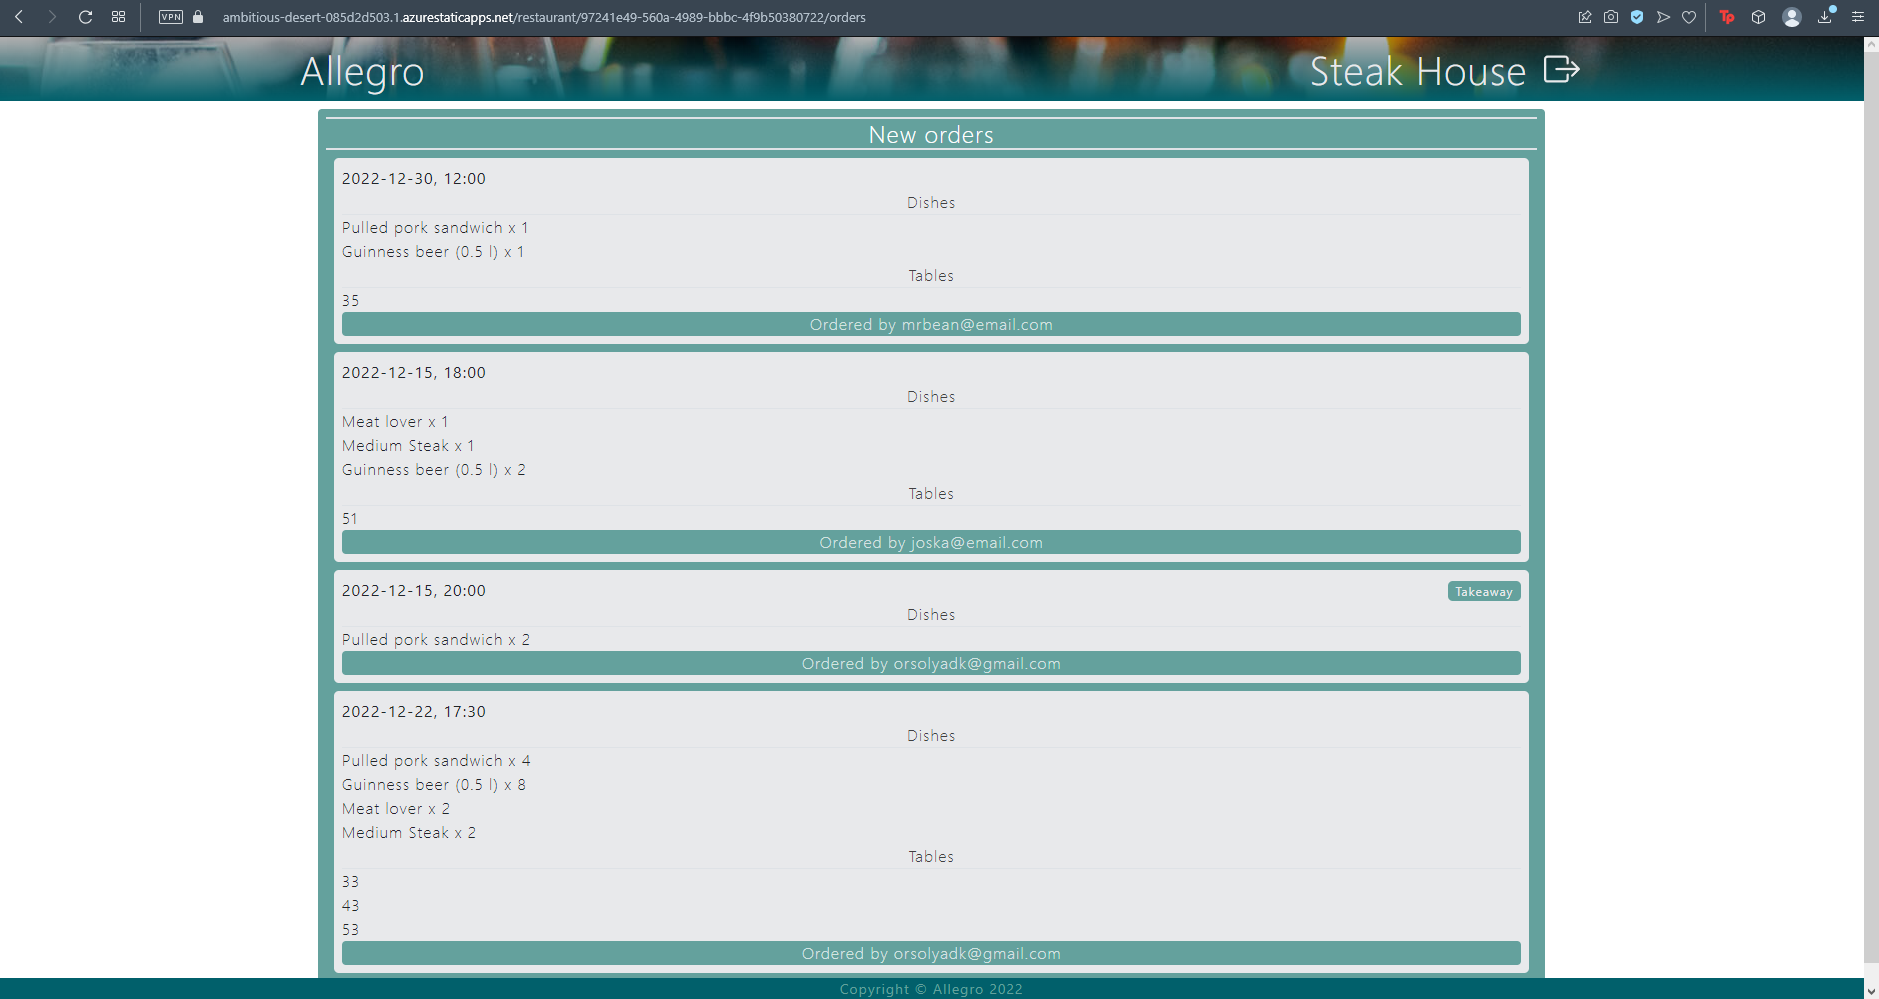
\includegraphics[width=150mm, keepaspectratio]{figures/UI/13_Orders.png}
	\caption{Restaurant all orders UI} 
	\label{fig:UI_13}
\end{figure}

\begin{figure}[ht]
	\centering
	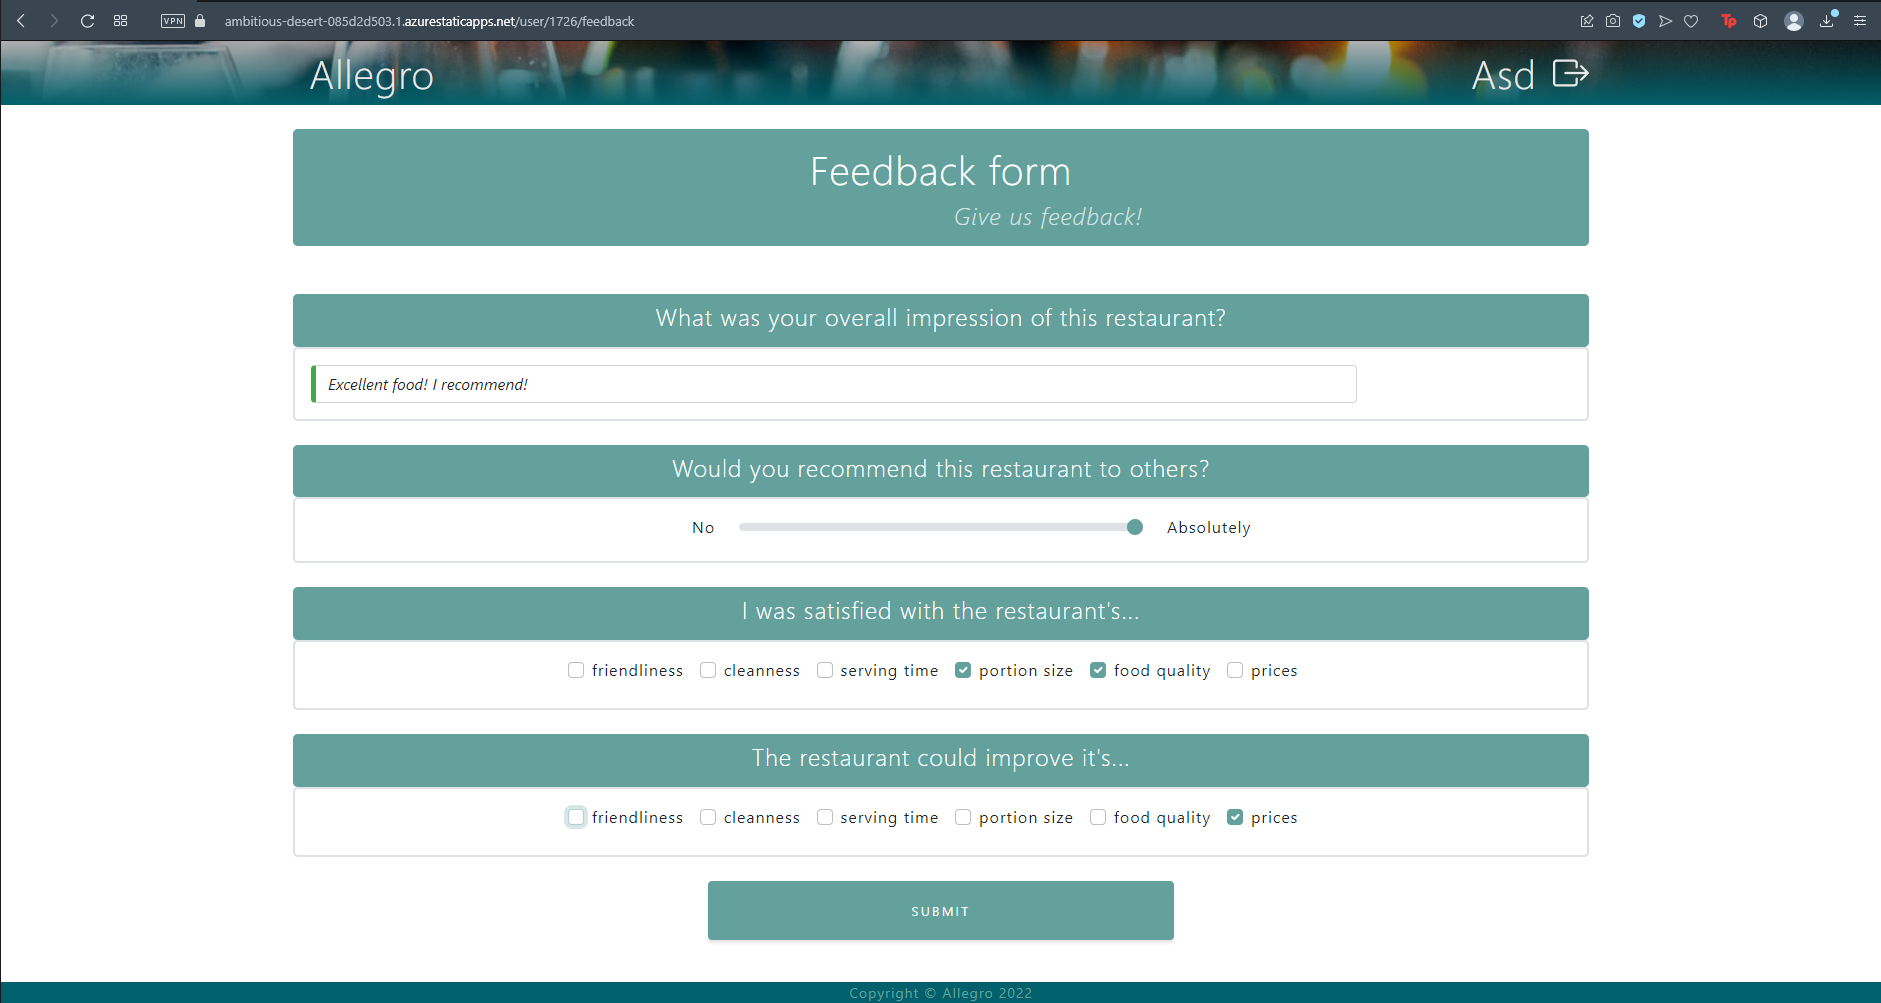
\includegraphics[width=150mm, keepaspectratio]{figures/UI/14_Feedback.png}
	\caption{Feedback component UI} 
	\label{fig:UI_14}
\end{figure}